\section{复频域分析}

\subsection{微分方程的变换解}

\begin{BoxDefinition}[微分方程的变换解]
    描述$n$阶系统的微分方程的一般形式为
    \begin{Equation}
        \sum\limits_{i=0}^{n}a_iy^{(i)}(t) = \sum\limits_{j=0}^{m}b_j f^{(j)}(t)
    \end{Equation}
    系统的初始状态为$y(0_{-}),y^{(1)}(0_{-}),\dots,y^{(n-1)}(0_{-})$。

    根据\xref{thm:拉普拉斯变换的微分定理},对方程两边微分
    \begin{Equation}
        \left[\sum\limits_{i=0}^{n}a_is^i\right]Y(s) - \sum\limits_{i=0}^{n}a_i
        \left[\sum\limits_{p=0}^{i-1}s^{i-1-p}y^{(p)}(0_{-})\right] = \left[\sum\limits_{j=0}^{m}b_js^j\right]F(s)
    \end{Equation}
    整理可得
    \begin{Equation}
        Y(s) = \frac{M(s)}{A(s)}+\frac{B(s)}{A(s)}F(s) = Y_{zi}(s)+Y_{zs}(s)
    \end{Equation}
    对$Y(s)$进行拉普拉斯逆变换即可得微分方程的全解。

    其中含衰减指数的项组成暂态分量\footnote{又叫自由响应,反应系统的固有频率}$y_t(t)$,其余的为稳态分量\footnote{又叫强迫响应,形式由激励函数确定}$y_s(t)$。
\end{BoxDefinition}

\subsection{系统函数}

\begin{BoxDefinition}[系统函数]
    定义系统函数
    \begin{Equation}
        H(s) = \frac{Y_{zs}(s)}{F(s)} = \frac{B(s)}{A(s)}
    \end{Equation}
    系统函数只与系统结构和元件参数有关,与激励和初始状态无关。

    根据系统函数可以求系统的零状态响应
    \begin{Equation}
        y_{zs}(t) = h(t)*f(t) \Rightarrow Y_{zs}(s) = \mathscr{L}\left[h(t)\right]F(s)
    \end{Equation}
    其中
    \begin{Equation}
        H(s) = \mathscr{L}\left[h(t)\right]
    \end{Equation}
\end{BoxDefinition}

\subsection{系统的s域框图}

\begin{Figure}[系统的s域框图]
    \begin{FigureSub}[s域加法器]
        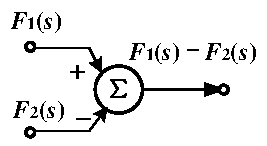
\includegraphics[width=40mm]{visio/5.4-a.pdf}
    \end{FigureSub}
    \begin{FigureSub}[s域积分器]
        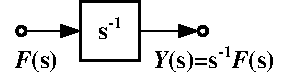
\includegraphics[width=40mm]{visio/5.4-b.pdf}
    \end{FigureSub}
    \begin{FigureSub}[s域数乘器]
        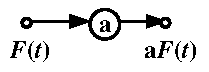
\includegraphics[width=40mm]{visio/5.4-c.pdf}
    \end{FigureSub}
\end{Figure}

由s域框图求微分方程方法与\xref{sec:系统的描述}相同,即设辅助函数$X(s)$作为激励输入处加法器输出,再写出$Y(s)$的表达式,最后用拉普拉斯逆变换即可。

\subsection{用拉氏变换法分析电路的步骤}

根据时域特性先列时域微分方程,再求其拉普拉斯变换,或直接根据电路的s域模型建立代数方程。

求解s域方程再做拉普拉斯逆变换即可。

\subsection{电路的s域模型}

\begin{BoxDefinition}[电阻元件的s域模型]
    \begin{Figure}[电阻元件的s域模型]
        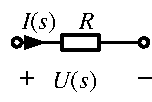
\includegraphics[width=30mm]{visio/5.5.pdf}
    \end{Figure}
    表达式
    \begin{Equation}
        u(t) = R i(t) \Rightarrow U(s) = R I(s)
    \end{Equation}
\end{BoxDefinition}

\begin{BoxDefinition}[电感元件的s域模型]
    \begin{Figure}[电感元件的s域模型]
        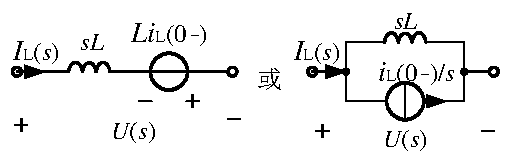
\includegraphics[width=70mm]{visio/5.6.pdf}
    \end{Figure}
    表达式
    \begin{Equation}
        U(s) = sLI_L(s) - Li_L(0_{-})
    \end{Equation}
    或
    \begin{Equation}
        I_L(s) = \frac{1}{sL}U(s)+\frac{i_L(0_{-})}{s}
    \end{Equation}
\end{BoxDefinition}

\begin{BoxDefinition}[电容元件的s域模型]
    \begin{Figure}[电容元件的s域模型]
        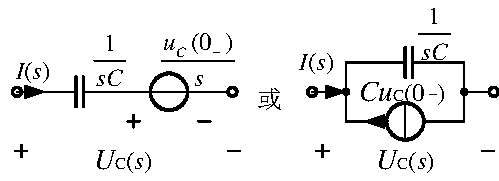
\includegraphics[width=70mm]{visio/5.7.pdf}
    \end{Figure}
    表达式
    \begin{Equation}
        I(s) = sCU_C(s) - Cu_C(0_{-})
    \end{Equation}
    或
    \begin{Equation}
        U_C(s) = \frac{1}{sC}I(s) + \frac{u_C(0_{-})}{s}
    \end{Equation}
\end{BoxDefinition}

\begin{BoxDefinition}[基尔霍夫定律的s域模型]
    基尔霍夫电流定律(KCL)
    \begin{Equation}
        \sum i(t) = 0 \Rightarrow \sum I(s) = 0
    \end{Equation}
    即节点电流代数和为零。

    基尔霍夫电压定律(KVL)
    \begin{Equation}
        \sum u(t) = 0 \Rightarrow \sum U(s) = 0
    \end{Equation}
    即回路电压代数和为零(要定电压参考方向,同向正反之负)。
\end{BoxDefinition}

求电路响应的步骤:

\begin{itemize}
    \item 画$0_{-}$等效电路,求初始状态
    \item 画s域等效模型
    \item 列s域方程(用节点分析法或网孔分析法,节点分析法设参考电位)
    \item 解s域方程,求响应的拉普拉斯变换$U(s)$或$I(s)$
    \item 用拉普拉斯逆变换求出$u(t)$或$i(t)$
\end{itemize}